\documentclass[a4paper]{article}

\usepackage[english]{babel}
\usepackage[utf8x]{inputenc}
\usepackage{amsmath}
\usepackage{amsfonts}
\usepackage{graphicx}
\usepackage[]{algorithm2e}
\usepackage[colorinlistoftodos]{todonotes}

\title{CS 5785 -- Applied Machine Learning -- Lec.\ 21}
\author{Prof.\ Nathan Kallus, Cornell Tech\\Scribe: TBD}
\date{Fall, 2017 (Under construction)}

\begin{document}
\maketitle

\section{Separating Hyperplanes - SVM}
Support Vector machine, SVMs for short, is one of the most common Machine Learning techniques. Recall that Logistic Regression and LDA are both methods that make some assumptions about the class densities and they just differ in the way the coefficients are estimated. At the time, we briefly discussed an alternative way to look at the problem in terms of separating line/plane/hyperplane, see Figure ~\ref{fig:414}. We also discussed generative vs discriminative methods, see Figure ~\ref{fig:murphyTable}. \\

\begin{figure}
\centering
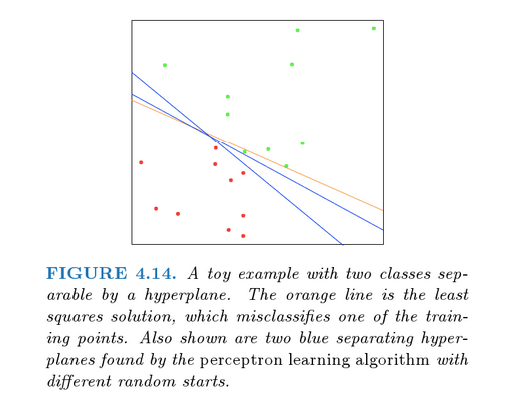
\includegraphics[width=0.75\textwidth]{fig414.png}
\caption{\label{fig:414}[HTF]}
\end{figure}

\begin{figure}
\centering
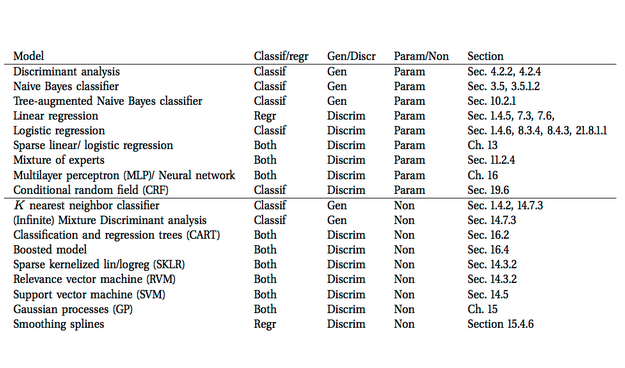
\includegraphics[width=0.75\textwidth]{murphyTable81.png}
\caption{\label{fig:murphyTable}[Murphy 8.1]}
\end{figure}

In some cases where the classes are separable, like in Figure~\ref{fig:414}, there are infinite number of possible solutions to the problem, i.e., lines that separate between the classes. We are interested in finding the best solution which is the most generalizable solution.

In Figure ~\ref{fig:414} the orange line represents the least squares fit which misclassifies one of the data points for response $Y\in\{1,-1\}$ on $X$:
$${x: \hat\beta_0+\hat\beta_1x_1+\hat\beta_2x_2=0}$$

Classifiers that compute a linear combination of input features and return the sign are sometimes called \textit{perceptrons}. Frank Rosenblatt, in 1958,  was the first to think of the idea of linear combinations of the input to represent the output, see Figure ~\ref{fig:frank}.

\begin{figure}
\centering
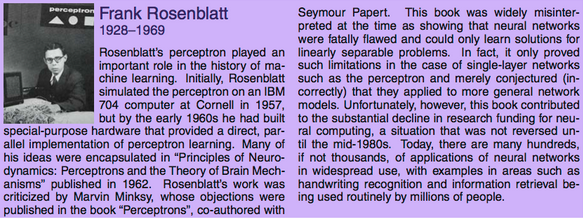
\includegraphics[width=0.75\textwidth]{frankRosenblat.png}
\caption{\label{fig:frank}[Bishop]}
\end{figure}

The Perceptron Learning algorithm tries to find a separating hyperplane by minimizing the distance of misclassified points to the decision boundary. This is a stepping stone to more advanced methods that deal with data that's not linearly separable.

First we need a quick review of some vector algebra. Figure ~\ref{fig:415} shows an \textit{affine set} $L$ (marked by the green line) defined by the equation:
$f(x)=\beta_0+\beta^\top x=0$ for  $x\in\mathbb{R}^2$. Think of $f(x)$ as a tilted plane intersecting the $(x_1,x_2)$ plane; this intersection is a line: on one side the values of $f(x)$ are positive, on the other negative, this leads to the notion of \textit{signed distance}.

\begin{figure}
\centering
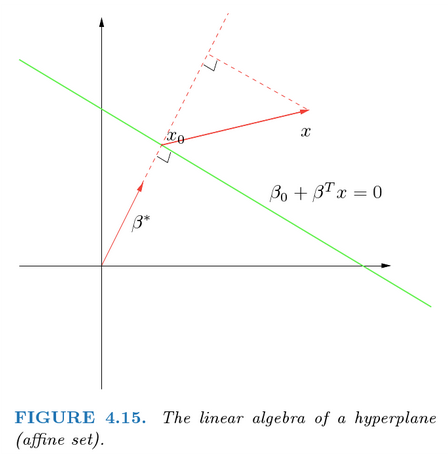
\includegraphics[width=0.75\textwidth]{fig415.png}
\caption{\label{fig:415}[HTF]}
\end{figure}

Properties:
\begin{enumerate}
\item For any $2$ points $x_1$ and $x_2$ lying in $L$, $\beta^\top (x_1-x_2)=0$, and hence $\beta^*=\frac{\beta}{\|\beta\|}$ is the unit vector normal to the surface $L$. Note that $L$ is the set of tips of vectors from the origin that have a dot product of $-\beta_0$ with $\beta$. Notice that $x_1-x_2$ is a vector parallel to $L$ and therefore has a dot product of $0$ with $\beta$.
\item For any point $x_0$ in $L$ we have that $\beta^\top x_0=-\beta_0$.
\item The signed distance between any point $x$ to $L$ is given by:
$$\beta^{*\top}(x-x_0)=\frac{1}{\|\beta\|}(\beta^\top x+\beta_0)=\frac{1}{\|f'(x)\|}f(x)$$
Hence $f(x)$ is proportional to the signed distance from $x$ to the affine set $L$ defined by $f(x)=0$. This is important because our observations, such as data points and training examples, are vectors in this space and we would like to characterize their relationship to $L$.
\end{enumerate}

\subsection{Perceptron Learning}
We will focus on Rosenblatt's perceptron learning algorithm, which finds a separating hyperplane by minimizing the distance of misclassified points to the decision boundary.

If a response $y_i=1$ is misclassified, then $x^\top\beta+\beta_0<0$, and the opposite for a misclassified response with $y_i=-1$

\begin{figure}
\centering
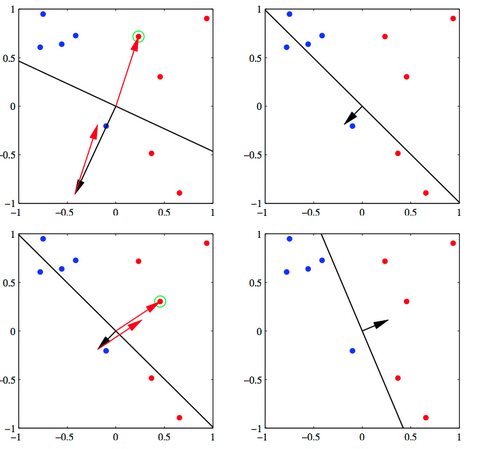
\includegraphics[width=0.75\textwidth]{bishop47.png}
\caption{\label{fig:bishop}From top left to bottom right. The black line represents represents the vector defined by $\beta$, a randomly generated starting point. The green marked red dot is a chosen misclassified point.[Bishop 4.7]}
\end{figure}

In Figure~\ref{fig:bishop} the perceptron algorithm is shown step by step, from the top left to the bottom right. We start with a random guess for $\beta$ and tweak the guess based on a randomly chosen misclassified point. In each step we add the signed distance between the origin and the red dot circled in green by placing the red vector at the tip of the black vector. We continue until there are no misclassifications. If the two classes are not linearly separable the algorithm would never stop, if the classes are linearly separable then the resulting boundary depends on the random guess we started with.

The goal is to minimize:
$$D(\beta, \beta_0)=-\sum_{i\in {\mathcal M}}y_i(x_i^\top\beta+\beta_0)$$
Where $\mathcal M$ is the set of misclassified points. $D(\cdot,\cdot)$ is nonnegative and proportional to the distance of the misclassified points to $L$ (defined by $\beta^\top x+\beta_0$). If we fix $\mathcal M$ the gradient is given by:
$$\frac{\partial D(\beta,\beta_0)}{\partial\beta}=-\sum_{i\in {\mathcal M}}y_ix_i$$
$$\frac{\partial D(\beta,\beta_0)}{\partial\beta_0}=-\sum_{i\in {\mathcal M}}y_i$$
Rosenblatt's algorithm uses \textit{Stochastic Gradient Descent} to minimize this piecewise linear criterion.

\subsection{Stochastic Gradient Descent (SGD)}

With SGD, instead of computing the sum of the gradient contributions of each observation followed by a step in the negative gradient direction, we take a step after each observation is visited. The missclassified observations are visited in some order (for example: random), and we update the parameters as follows:
$$\left(\begin{array}{cc}
\beta \\
\beta_0 \\
\end{array}\right)\leftarrow
\left(\begin{array}{cc}
\beta \\
\beta_0 \\
\end{array}\right)+\rho
\left(\begin{array}{cc}
y_ix_i \\
y_i \\
\end{array}\right)$$
$\rho$ is called the \textit{learning rate}. Let $\rho=1$ w.l.o.g. The errors ``kick around'' the hyperplane until it stabilizes, as seen in Figure ~\ref{fig:bishop}. If the classes are linearly separable one can show that the algorithm converges to a separating hyperplane in a finite number of steps. There are some problems that arise:

\begin{itemize}
\item For separable data, we have many solutions, and the one found depends on our initialization of the algorithm.
\item The finite number of steps can be very large. The smaller the gap, the more time to find it.
\item For non-separable data, the algorithm won't converge and cycles -- possibly quite long and, as such, hard to detect -- can develop.
\end{itemize}

One way to address the second problem (the number of steps) is to ``lift'' the data out of the original space via some sort of basis-function transformations, and seek a hyperplane in that space. This may risk overfitting.
Let's consider the XOR problem:
$$\begin{array}{cc}
\times & \circ \\
\circ & \times \\
\end{array}$$

This is clearly not linearly separable with any line. So how can we linearly separate these two classes? By moving the problem into a higher dimension, we can magically make it linearly separable. The way to choose the added dimension is by a \textit{kernel}.

So now that we can ``force'' data to be linearly separable we need a way to find the best separator.

\subsection{Optimal Separating Hyperplanes}
In 1996, Vapnik said that we should add the constraint of maximizing the distance to the closest point from either class in order to find the optimal hyperplane. By \textit{maximizing the margin} between the two classes on the training data, we get better classification performance on the test data, see Figure ~\ref{fig:416}.\\

\begin{figure}
\centering
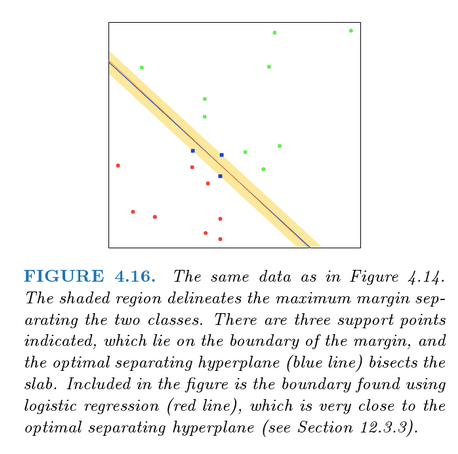
\includegraphics[width=0.75\textwidth]{fig416.png}
\caption{\label{fig:416}The yellow area represents the margin on each side of the boundary. [HTF]}
\end{figure}

Let's revisit $D(\beta,\beta_0)$ with this in mind. Consider the optimization criterion:
$$\max_{\beta,\beta_0,\|\beta\|=1} M$$
Subject to $$y_i(x_i^\top\beta+\beta_0)\geq M$$
For $i=1,2,\ldots,N$. This ensures that all points are a signed distace $M$ from the decision boundary defined by $(\beta,\beta_0)$, and we seek the largest such $M$. We can absorb the $\|\beta\|=1$ constraint by writing the conditions as:
$$\frac{1}{\|\beta\|}y_i(x_i^\top\beta+\beta_0)\geq M$$
By doing that we essentially redefine $\beta_0$. Equivalently, we could state the constraint as:
$$y_i(x_i^\top\beta+\beta_0)\geq M\|\beta\|$$
Since for any $\beta$ and $\beta_0$ satisfying this inequality, any positively scaled multiple also satisfies it. We can arbitrarily set $\|\beta\|=\frac{1}{M}$ and replace our maximizing problem with the following minimizing problem:
$$\min_{\beta,\beta_0}=\frac{1}{2}\|\beta\|^2$$
Subject to $$y_i(x_i^\top\beta+\beta_0)\geq 1$$
For $i=1,2,\ldots,N$.

These constraints define an empty ``slab'' or margin around the linear decision boundary of thickness $\frac{1}{\|\beta\|}$. This is a convex optimization problem. It is a quadratic criterion with linear inequality constraints. The Lagrange (primal) function, to be minimized with regard to $\beta$ and $\beta_0$ is:
$$L_p=\frac{1}{2}\|\beta\|^2-\sum_{i=1}^N\alpha_i[y_i(x_i^\top\beta+\beta_0)-1]$$
This basically takes the constraint and turns it into weighted penalties.


\begin{figure}
\centering
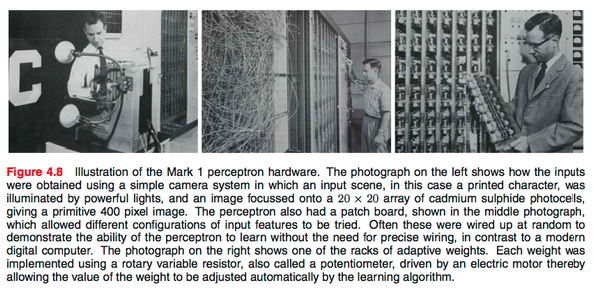
\includegraphics[width=0.75\textwidth]{bishop48.png}
\caption{\label{fig:bishop48}[Bishop]}
\end{figure}


\section{Deriving the SVM}

To solve this problem, set the derivative with respect to $\beta_1$, $\beta_0$ equal to zero.

\begin{align}
\beta &= \sum_{i=1}^{N} \alpha_i y_i x_i\\
0 &= \sum_{i=1}^{N} \alpha_i y_i
\end{align}

Recall that $\|\beta\|^2 = \beta^\top \beta$. So $\frac{1}{2} \frac{d}{d\beta} \|\beta\|^2 = \beta$ thinking about doing a derivative with vectors.  This is telling us that the coefficients are a linear combination of all observations weighted by $\alpha$ and the label.  If you plug $\beta$ back into the expression for $L_p$ you get the ``Wolfe dual'':

\begin{align}
L_D = \sum_{i=1}^{N} \alpha_i - \frac{1}{2} \sum_{i=1}^{N} \sum_{k=1}^{N} \alpha_i x_k y_i y_k x_i^\top x_k \;
\text{ subject to } \alpha_i \geq 0
\end{align}

The $x_i^\top x_k$ in the above equation is an inner product that can be swapped in for a kernel instead, which is a generalization of a dot product.

We get the solution by maximizing $L_D$ in the \emph{positive orthant}, i.e., $\alpha_i \geq 0$, a simple convex optimization problem for which standard solvers can be used.

The solution must also satisfy the Karush-Kuhn-Tucker (KKT) conditions which consist of Equations (1), (2), (3), and below (4).

\begin{align}
\alpha_i [y_i (x_i^\top \beta + \beta_0) -1] = 0 \; \forall i
\end{align}

This tells us that:
\begin{enumerate}
\item If $\alpha_i > 0$ then $y_i (x_i^\top \beta + \beta_0) =1$, i.e. $X_i$ is on the boundary of the slab, as seen in Fig. ~\ref{fig:svm1}. 
\item If $y_i (x_i^\top \beta + \beta_0) > 1$, $x_i$ is not on the boundary of the slab, and $\alpha_i=0$.
\end{enumerate}

\begin{figure}
\centering
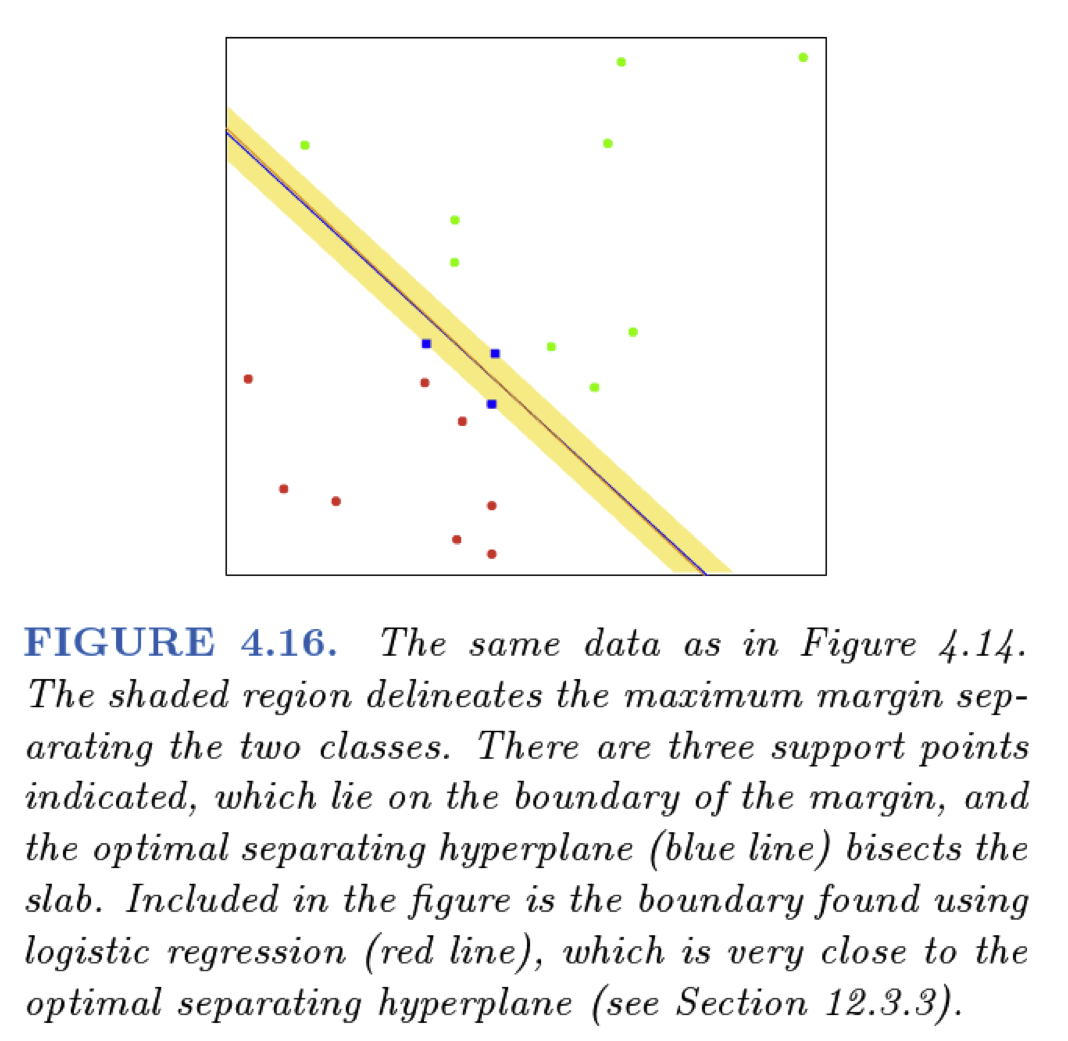
\includegraphics[width=1.0\textwidth]{fig4_16.png}
\caption{\label{fig:svm1}Figure 4.16}
\end{figure}

From Equation (1) we see that $\beta$ is defined as a linear combination of the support points $\alpha_i$.

We get $\beta_0$ by solving for Equation (4) for any of the support points.  Finally, the optimal separating hyperplane is given by:

\begin{align*}
\hat{f}(x) &= x^\top \beta + \beta_0 \\
\hat{G}(x) &= sign \; \hat{f}(x)
\end{align*}

Every point in the data set has the potential to have a non-zero $\alpha$ but the data points that contribute to the separating hyperplane are the ones on the margin, on the periphery of the slab.  This is extremely efficient since most of the points are zero and don't contribute to the decision.  You get $\beta$ and the offset $\beta_0$ and then threshold it to get the final decision.

Let's compare this with LDA and logistic regression, assuming a 2-class problem that's separable.  For LDA, we assume the classes are distributed as bivariate Gaussians that have the same means but different covariances.  But it's probably not the case that your data is like this  For logistic, you also get a decision line or hyperplane using not the points themselves but with log-odds as a linear combination.  Logistic is pretty similar qualitiatively to SVM because we get driven to two extreme values.  In Newton-Raphson, the coefficents are most important close to the boundary.  All points become support vectors or not, so $\alpha=0$ or $\alpha \neq 0$.

\section{Non-separable Hyperplanes}

What do you do when the data is not separable (not some slab away from a hyperplane)?

\begin{figure}
\centering
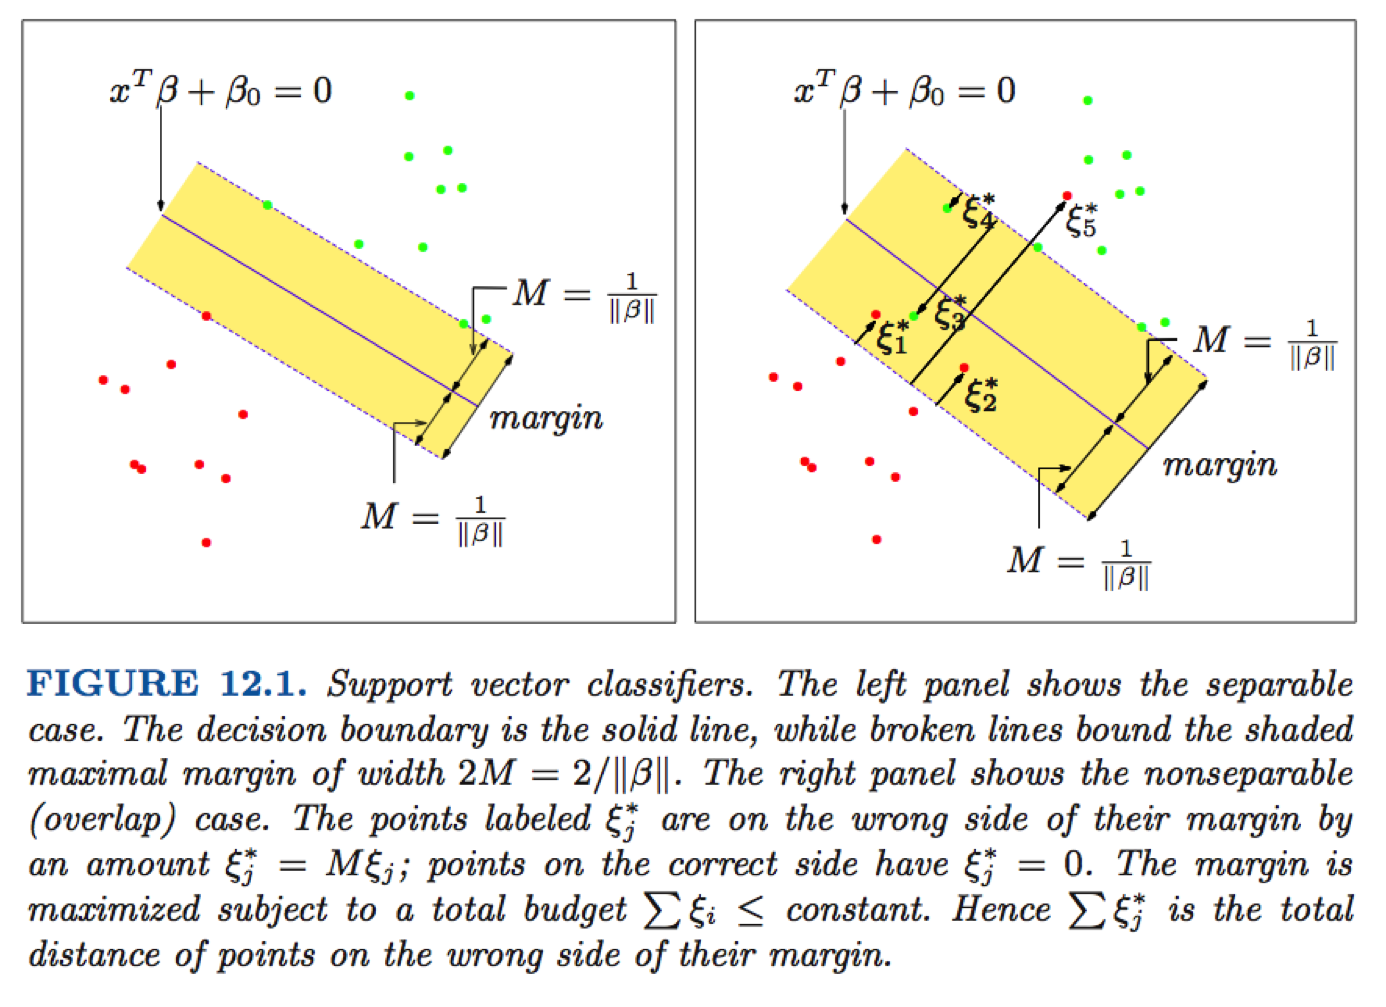
\includegraphics[width=1.0\textwidth]{fig12_1.png}
\caption{\label{fig:svm2}Figure 12.1}
\end{figure}

We won't do derivations for this non-separable case but we will talk about this, as seen in ~\ref{fig:svm2}.  When you look at the non-separable case, you think that have a margin that is a perfectly separating margin and have some points on the wrong side of the boundary.  You attach to every single data point a \textit{slack variable}, $\xi_i$.  The slack variable has the ability to move into the correct side like a rubber band, if you're willing to pay the price.

However, we may overfit if the slack variables are left unconstrained.  The amount of stretch is specified by the variable $c$, a regularization constant or cost, which we last saw with decision trees.  We want a compromise allowing some data points to have slack.  The regularization is like having a budget for the slack variables.  If $c=0$ then you're not constraining anything.  If $c$ is really big, you're being very inflexible assuming that nothing is allowed to violate the constaint, on the left, which is very inflexible.  You can use cross-validation to find c.  Fig. ~\ref{fig:svm3} shows an example.

\begin{figure}
\centering
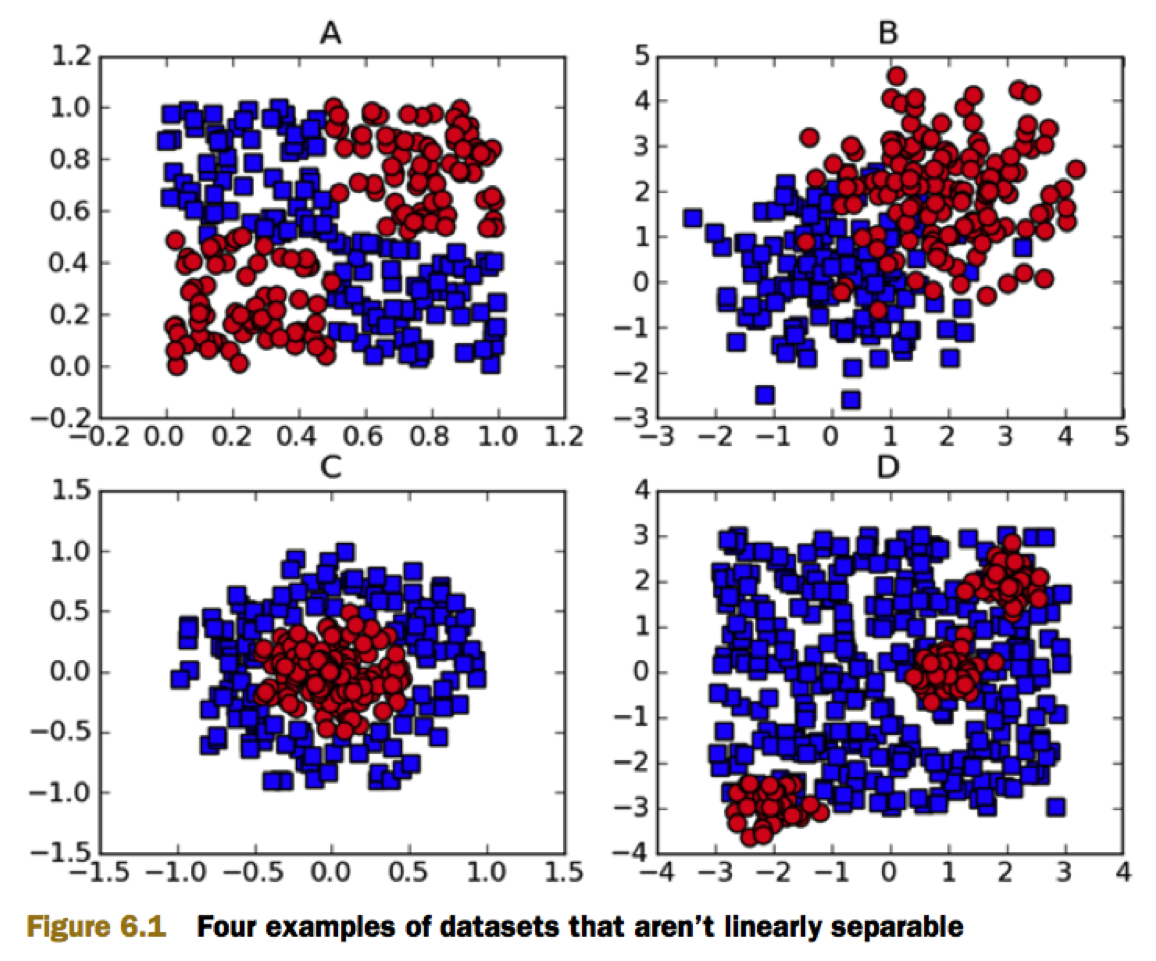
\includegraphics[width=1.0\textwidth]{fig6_1.png}
\caption{\label{fig:svm3}Figure 6.1}
\end{figure}

Support-vector machines let you visualize the prototypes that sit $\pm \epsilon$ around the boundary.  For images, When a new face comes in, it's quite efficient with SVM.  For kNN you would have to compute the distances to every single face.  In SVM, you bring in the new face and do an inner product with the support vectors and if you look at sex classifications for faces in Fig. ~\ref{fig:svm4} you see that these two faces are just $\epsilon$ more or less feminine or masculine.  You can see these exemplars.

A linear SVM probably isn't powerful enough to calculate this.  We need a mechanism to bring in more powerful notions of similarity between patterns.

\begin{figure}
\centering
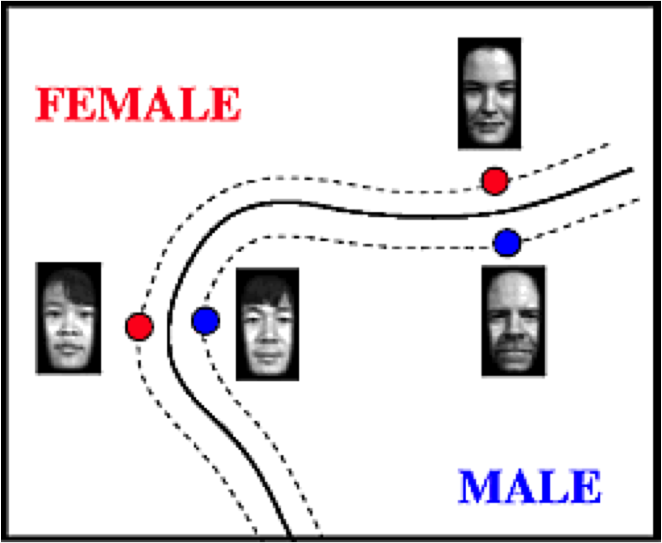
\includegraphics[width=1.0\textwidth]{male_female.png}
\caption{\label{fig:svm4}Male Female}
\end{figure}

\section{Kernels}

What is a kernel? A kernel is a function that satisfies the following conditions:
$$
\sum_{i,j} k(x_i, x_j) c_i c_j \geq 0
$$
for some set of feature vectors $\{x_i\}$ and any vector $c$.

We say the kernel is ``Mercer'' or that it is positive semidefinite. If this were just:
$$
\sum_{i,j} A_{ij} c_i c_j \geq 0
$$
or equivalently
$$
c^\top A c \geq 0 \; \text{because positive semidefinite} \; A = QQ^\top
$$

If a matrix is positive semidefinite, we can write it as a product of a matrix with its transpose.  Also each entry in a positive semidefinite matrix can be expressed by the pairwise inner products of a set of vectors.

$$
k(x,y) = \phi(x) \cdot \phi(y)
$$

The kernel function, $k(\cdot,\cdot)$, is operating on all data points and pops out numbers for all possible pairs.  If the resulting matrix satisfies the Mercer condition, that means the function $k$ represents an inner product between two vectors. We're generalizing the dot product so if it satisfies this condition, there exists some features vectors that give you the number by computing $k$.  

This is called the ``kernel trick''.  So if you learn a method built around inner products, you look at the algorithm and everywhere it has a dot product, you pull in a kernel instead.  That means you do the algorithm on a higher-dimensional version of the data instead of the data itself.

Whatever $k(x,y)$ is doing, you're lifting the vector into a higher dimensional feature space by using  $ \phi(\cdot)$, and computing  the inner product between $ \phi(x)$ and $ \phi(y)$. 

Let's say $\phi(x)$ represents an empirical feature mapping:
$$
\phi: (x_1, x_2)^\top \rightarrow (x_1, x_2, x_1^2-x_2^2)^\top
$$
$$
x \in {\rm I\!R}^2, \phi(x) \in {\rm I\!R}^3
$$

Here we went from the native data that is 2-dimensional to mapped 3-dimensional data, supplemented by the sum of squares. $\phi$ is implicit. You just choose the kernel.

If you imagine a clump with an annulus, the data may not be perfectly linearly separable but by adding a dimension becomes more separable, perhaps with a plane.

\subsection{Examples of Kernels}

\begin{enumerate}
\item
RBF (radial basis function):
$$
k(x,y) = e^{-{\| x-y \|}^2 / \alpha}
$$

\item For histogram data $h_i, g_i$, use $\chi^2$ kernel:
$$
\chi^2 = \frac{1}{2} \sum_{i=1}^{K} \frac{{(h_i-g_i)}^2}{h_i+g_i}
$$
$$
k(h,g) = e^{-\chi^2(h,g) / \alpha}
$$
\end{enumerate}

	3. Trivial Kernel (dot product)
    $$k(x,y) = x^Ty$$
There is some $\phi(x)$ that would give you a new vector that if you do the inner product on would give you the same as the kernel.  However, some of these feature mappings would be infinitely long.  

\begin{figure}
\centering
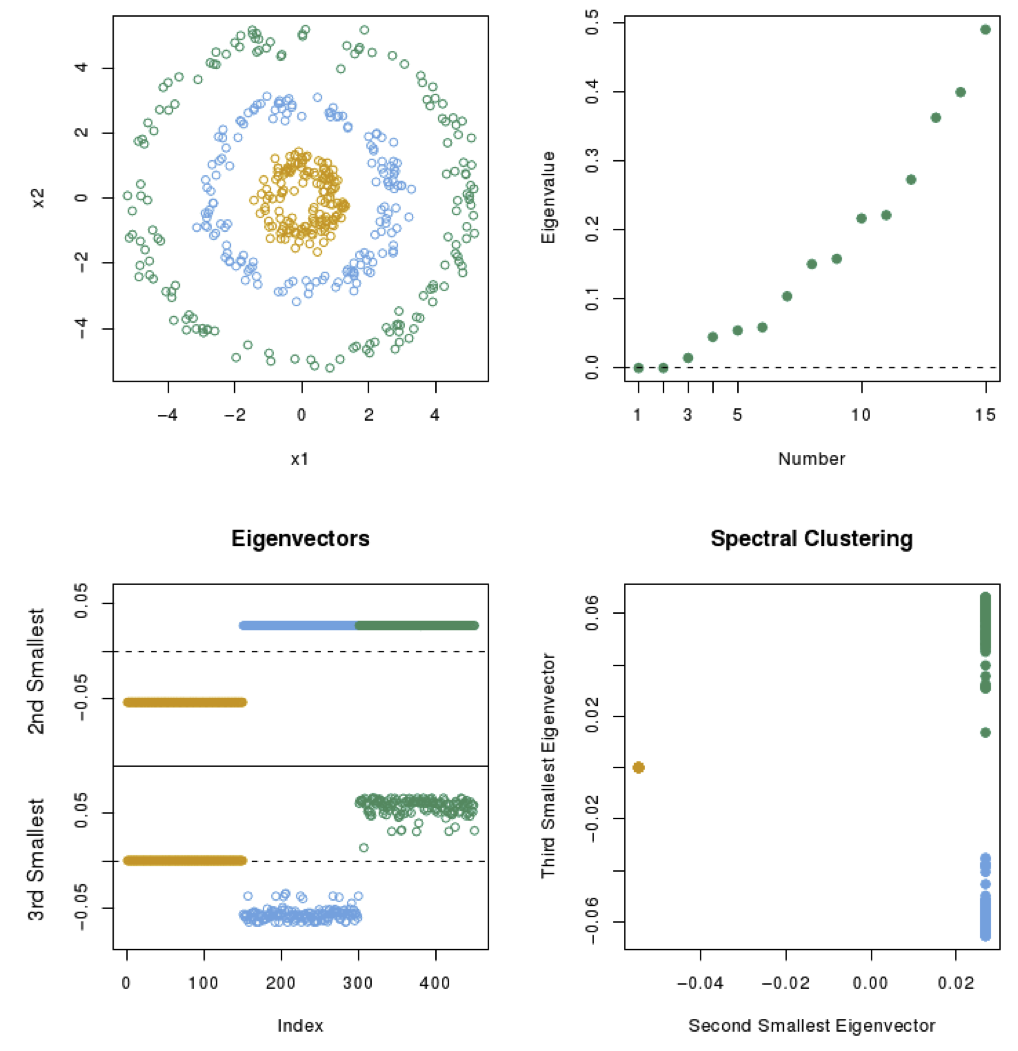
\includegraphics[width=1.0\textwidth]{fig14_29.png}
\caption{\label{fig:kernel}Fig. 14.29}
\end{figure}

The main place you see these things is with SVMs with kernels, kPCA, and spectral clustering.  We can see some of this in Fig. ~\ref{fig:kernel}.  

If you did K-Means with the top left you probably wouldn't get anything useful.  With spectral clustering, you still use K-Means but first evaluate a Gaussian between all pairs of points, creating a kernel matrix using one of the example kernels above.  You get a Gaussian-weighted distance matrix and find its leading eigenvectors and keep the first k.  If you plot the eigenvectors and keep the first k, you do K-Means and then get this nice separation between the clusters.  The first eigenvector separates from the second and the second separates the third.  You still use k-means after producing the kernel matrix and its eigenvectors.  You do clustering on the leading eigenvectors.


\end{document}
